\documentclass[11pt]{article}
\usepackage{subfigure,wrapfig,graphicx,booktabs,fancyhdr,amsmath,amsfonts}
\usepackage{bm,amssymb,amsmath,amsthm,wasysym,color,fullpage,setspace,multirow}
\usepackage{listings, xcolor}
\usepackage{pdfpages}
\usepackage{siunitx}
\usepackage[margin=1in]{caption}
\captionsetup[figure]{font=small,labelfont=small}


\title{ASE 389P.4 Methods of Orbit Determination \\ Final Project Submission}
\author{Corey L Marcus} \date{Wednesday, May 12\textsuperscript{th}}

%command to write C++ nicely
\def\CC{{C\nolinebreak[4]\hspace{-.05em}\raisebox{.4ex}{\tiny\bf ++}}}

%commands to include C++ code in appendix
\lstset { %
	language=C++,
	backgroundcolor=\color{black!5}, % set backgroundcolor
	basicstyle=\tiny,% basic font setting
}

\begin{document}
\onehalfspace
\maketitle

\abstract{This project showcases the skills learned during the Orbital Determination course. The estimation scheme involves a nonlinear least-squares based estimator initialization followed by a standard Unscented Kalman Filter.}

\section{Introduction}

This report documents the final project. We are provided approximately 6 days of satellite range and range-rate measurements from three ground based stations. Our objective is to use these measurements to deliver a satellite state estimate seven days after the initial epoch. \\

The following sections document the methodology used, including system dynamics modeled, approximations made, and estimation schemes used. Then deliverables are displayed and discussed. Finally, estimator performance is evaluated.

\section{Methodology}

\subsection{System Dynamics}

This subsection details the system dynamics used to model the spacecraft's orbit. All code was written in {\CC} for its increased speed when compared to scripting languages such as MATLAB. Many of the algorithms used were sourced from the well-known text "\textit{Fundamentals of Astrodynamics and Applications}" by David Vallado.

\subsubsection{Gravity Model}

An EGM-96 gravity model was used up to a 20x20 gravity field. The choice to use {\CC} was motivated primarily by the computational expense of this gravity model. A slower language such as MATLAB would have much longer propagation times for the same complexity gravity model.

\subsubsection{Drag Model}

A simple cannonball drag model was used due to the relatively small effect of drag on the spacecraft's orbit. The cross-sectional area of the spacecraft was approximated at \SI{22}{\meter\squared} and the coefficient of drag at 1.88.

\subsubsection{Solar Radiation Pressure Model}

Similar to atmospheric drag, a simple cannonball model was used to model Solar Radiation Pressure (SRP). SRP force is not modeled when the spacecraft is shielded from the sun by the Earth's shadow. The coefficient of drag for SRP was approximated as 0.1. It was noted that the system had a very low sensitivity to SRP so limited effort was applied to its estimation and modeling.

\subsubsection{Luni-Solar Model}

Third body gravitational effects from the Sun and Moon were included. The acceleration due to each of these bodies was found according to a simple point-mass gravitational model. This simplification is justified due to the significant distance between the spacecraft and each of the third bodies. Algorithms to locate the Sun and Moon as a function of the current UTC time were found in \textit{Vallado}.

\subsection{Measurement Model}

A standard range and range-rate measurement model were used to generate predicted measurements. One difficulty is that the speed of light must be accounted for in determining when to utilize a measurement. Noting that the signal to noise ratio of the range measurements is extremely high, the measurement was used directly along with the speed of light in determining its time of flight. The measurement update was therefore applied at the time of receipt minus the time of flight. This time of flight was also used to account for aberration effects in the measurement model. \\

Measurement biases were estimated by running the estimator while considering measurements from only two of the three stations. A measurement bias was found for one of the stations and is discussed in a following section.

\subsection{Estimation}

The estimation scheme centers around an Unscented Kalman Filter (UKF). The UKF is a nonlinear extension of the standard Kalman Filter. Its hallmark is approximation of covariances in the propagation and update phase through numerical propagation of a collection of sigma points chosen to conveniently represent the distribution of the prior. After propagation through time or into the measurement space, approximations of the mean and variance of the transformed distribution can be found by investigating the spacial distribution of the sigma points. It was chosen over the more traditional Extended Kalman Filter (EKF) because it does not require explicit computation of the state-transition matrix. The true STM in this case is complex mathematically and computationally. Approximations of the STM would not serve us well over the long intervals without measurements. \\

A ``$2n+1$" number of points were used along with a single tuning parameter $k=0.5$. This value was chosen so that all sigma points would be given the same weight. \\

Filter initialization is a challenge for many nonlinear extensions of the Kalman Filter. Improper initialization can quickly lead to filter divergence. A nonlinear least-squares optimization scheme was used to find the initial state estimate. This involved using Levenberg-Marquardt (LM) to select the initial state, $x_0$, such that the norm of the prefit residuals, Equation \eqref{eq:ICcost}, was minimized. To reduce the computational complexity, only the first 50 measurements were considered. In Equation \eqref{eq:ICcost} $f_a^b(\cdot)$ represents the nonlinear propagation of the satellite's state from the time of measurement $a$ to $b$, $h(\cdot)$ represents the measurement dynamics, and $z_i$ represents the $i$\textsuperscript{th} measurement. 

\begin{equation}
	\label{eq:ICcost}
	J(x_0) = \sum_{i=0}^{i=50} \left( z_i - h(f_{0}^{i}(x_0)) \right)^2 
\end{equation}

The resulting $x_0$ is shown in Equation \eqref{eq:LM_IC}. The units are $km$ and $km/s$. The initial estimate covariance, $P_0$, was chosen arbitrarily to achieve a filter which converged for all test cases. This matrix is shown in Equation \eqref{eq:P0}. To correspond with the state, the units are $km^2$ and $km^2/s^2$. $diag \{a, b, c, ... \}$ is shorthand for a diagonal matrix with its arguments on the diagonal.

\begin{equation}
	\label{eq:LM_IC}
	x_0 = \begin{bmatrix}
	6980.3967323588 \\
	1619.61802198332 \\
	15.1399428739289 \\
	-1.66690187359566 \\
	7.2578409459164 \\
	0.261907498000759 \\	
	\end{bmatrix}
\end{equation}

\begin{equation}
	\label{eq:P0}
	P_0 = diag \{ 100, 100, 100, 0.01, 0.01, 0.01 \}
\end{equation}

The choice was made to estimate only position and velocity due to the limited quality of the dynamics model. If items such as coefficient of drag and solar radiation pressure are to be estimated, a much higher quality model with lower process noise is needed due to rather weak observability of these quantities. \\

An unsuccessful attempt was made to use the LM optimizer to find an estimate of the drag coefficient but did not prove fruitful. When attempting to optimize $C_d$, the system rapidly increases $C_d$ towards infinity for unknown reasons. Further investigation is needed in this area to improve estimator performance. \\

Another unsuccessful attempt was made to estimate $C_d$ with the UKF. The coefficient appears to be very weakly observable as its estimate variance does not decrease significantly and the estimate wanders back and forth between positive and negative numbers. An inspection of the covariance matrix between the state $x$ and measurement $y$, $P_{xy}$ shows zero correlation between the $C_d$ and measurement with my model (bottom row of $P_{xy}$). This implies that $C_d$ is unobservable for a single measurement. It is likely to be only weakly observable through multiple measurements. This is the main reason I have so much trouble estimating $C_d$. $P_{xy}$ for the initial measurement is shown below in Equation \eqref{eq:P_xy}.

\begin{equation}
\label{eq:P_xy}
P_{xy} = \begin{bmatrix}
    6.6535081737267152 & 0.0095716394089781307 \\
   -6.1555964033719874 &  0.018602911245598531 \\
    4.2235397458787887 &  0.012033468766868966 \\
                     0 & 0.0066535427968655476 \\
                     0 & -0.0061556321012348463 \\
1.3552527156068805e-20 & 0.0042235721474275702 \\
                     0 &                     0
\end{bmatrix}
\end{equation}


Process noise is an important component of estimation used to account for unmodeled dynamics and inputs to the system. The process noise covariance, $Q$, was modeled according to the suggestion in the Final Project Assignment and is shown in Equation \eqref{eq:Q}. Process noise was applied in the RIC frame to because uncertainties in drag tend to manifest primarily in the in-track direction. The size of the components $\sigma_R^2$, $\sigma_I^2$, $\sigma_C^2$ were chosen manually to produce adequate filter performance. These values was found to be: $\sigma_R = 1$E$-10$ km, $\sigma_I = 1$E$-9$ km, and $\sigma_C = 1$E$-10$ km.

\begin{equation}
\label{eq:Q}
Q = \Delta t^2 \begin{bmatrix}
\frac{\Delta t^2}{4} \sigma_R^2 & 0 & 0 & \frac{\Delta t}{2} \sigma_R^2 & 0 & 0 \\
0 & \frac{\Delta t^2}{4} \sigma_I^2 & 0 & 0 & \frac{\Delta t}{2} \sigma_I^2 & 0 \\
0 & 0 & \frac{\Delta t^2}{4} \sigma_C^2 & 0 & 0 & \frac{\Delta t}{2} \sigma_C^2 \\
\frac{\Delta t}{2} \sigma_R^2 & 0 & 0 & \sigma_R^2 & 0 & 0 \\
0 & \frac{\Delta t}{2} \sigma_I^2 & 0 & 0 & \sigma_I^2 & 0 \\
0 & 0 & \frac{\Delta t}{2} \sigma_C^2 & 0 & 0 & \sigma_C^2 \\	
\end{bmatrix}
\end{equation}

No parameters were considered by my estimation scheme and no smoothing was performed.

\section{Deliverables}

\subsection{Prefit Residuals}

Figure \ref{fig:prefit} shows the prefit measurement residuals when all measurement types and sensors are considered. To better demonstrate detail Figure \ref{fig:prefit_zoom1} shows a zoomed-in plot of the measurement residuals.

\begin{figure}[!htb]
	\centering
	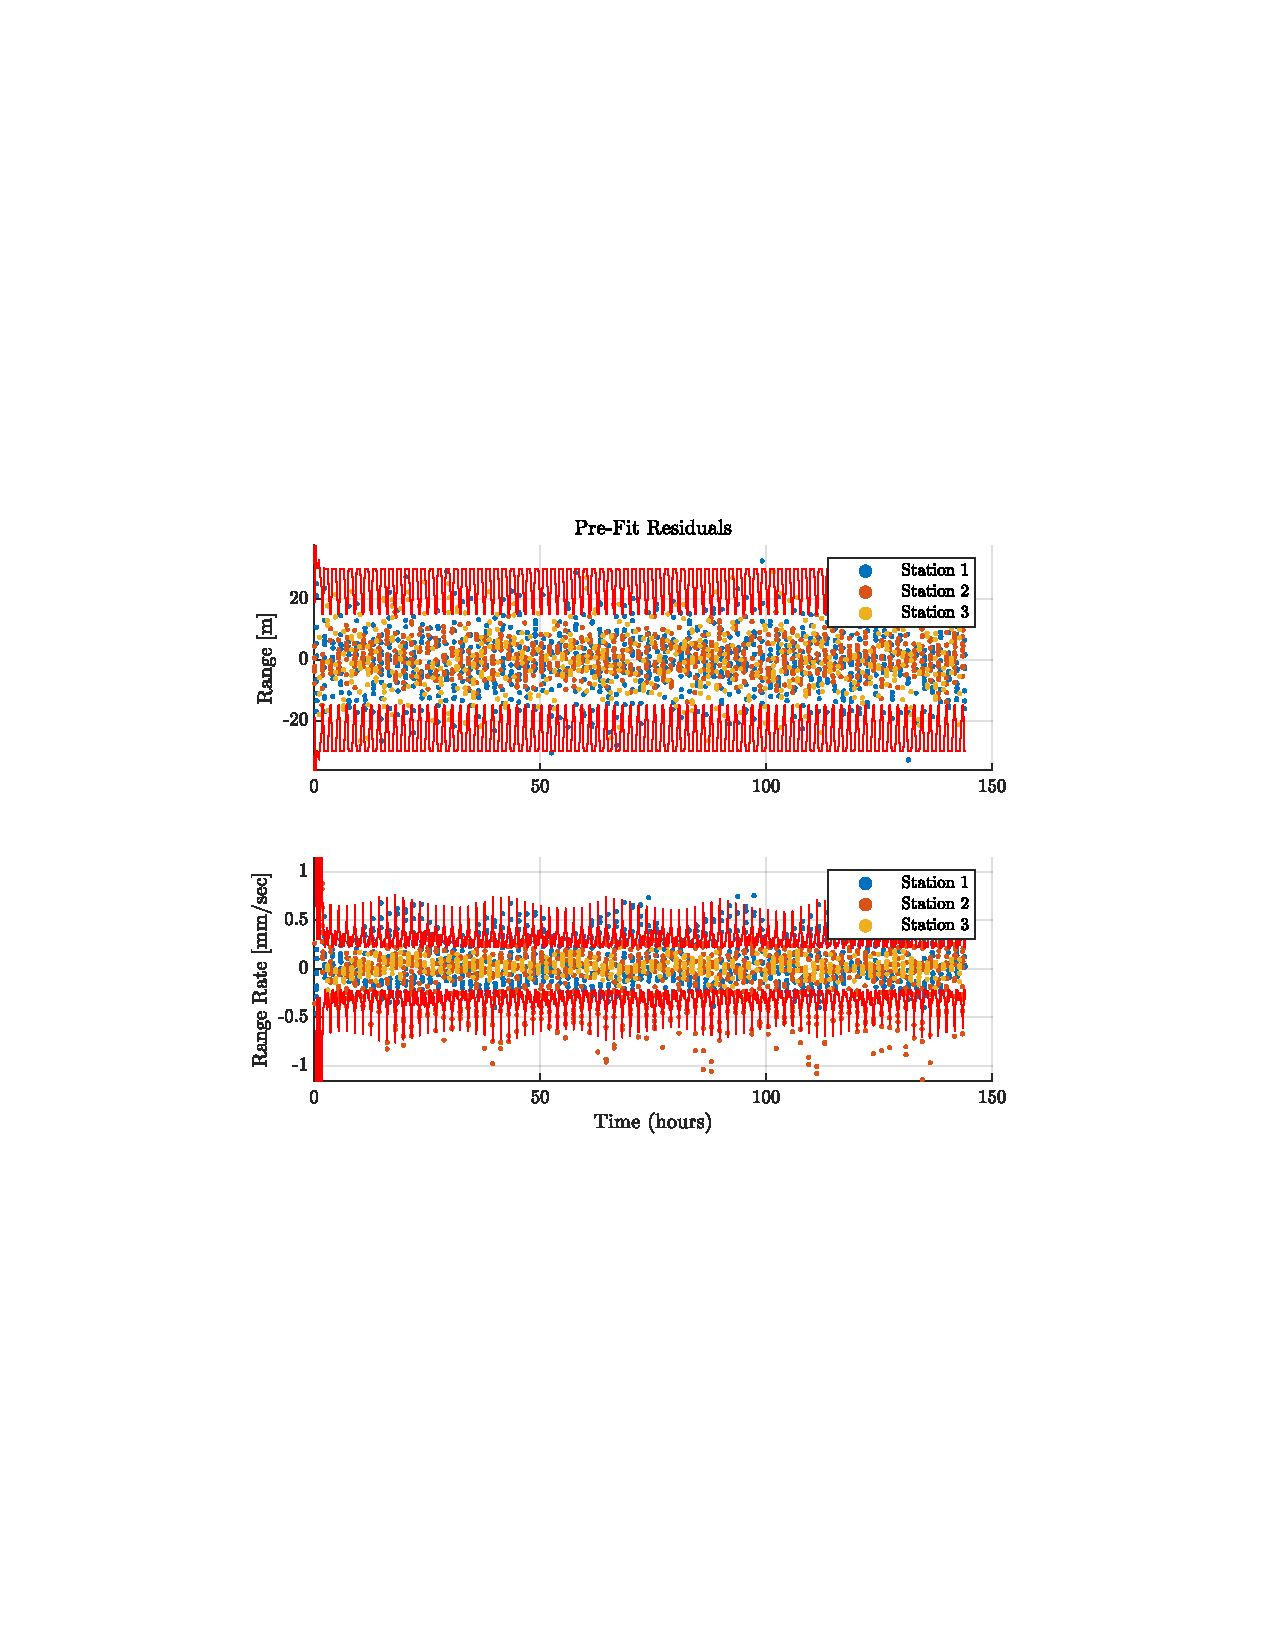
\includegraphics[clip,trim=4cm 8.5cm 4cm 8.5cm, width=.5\textwidth]{figs/prefit_res_final.pdf}
	\caption{The prefit measurement residuals for range (top) and range-rate (bottom).}
	\label{fig:prefit}
\end{figure}

\begin{figure}[!htb]
	\centering
	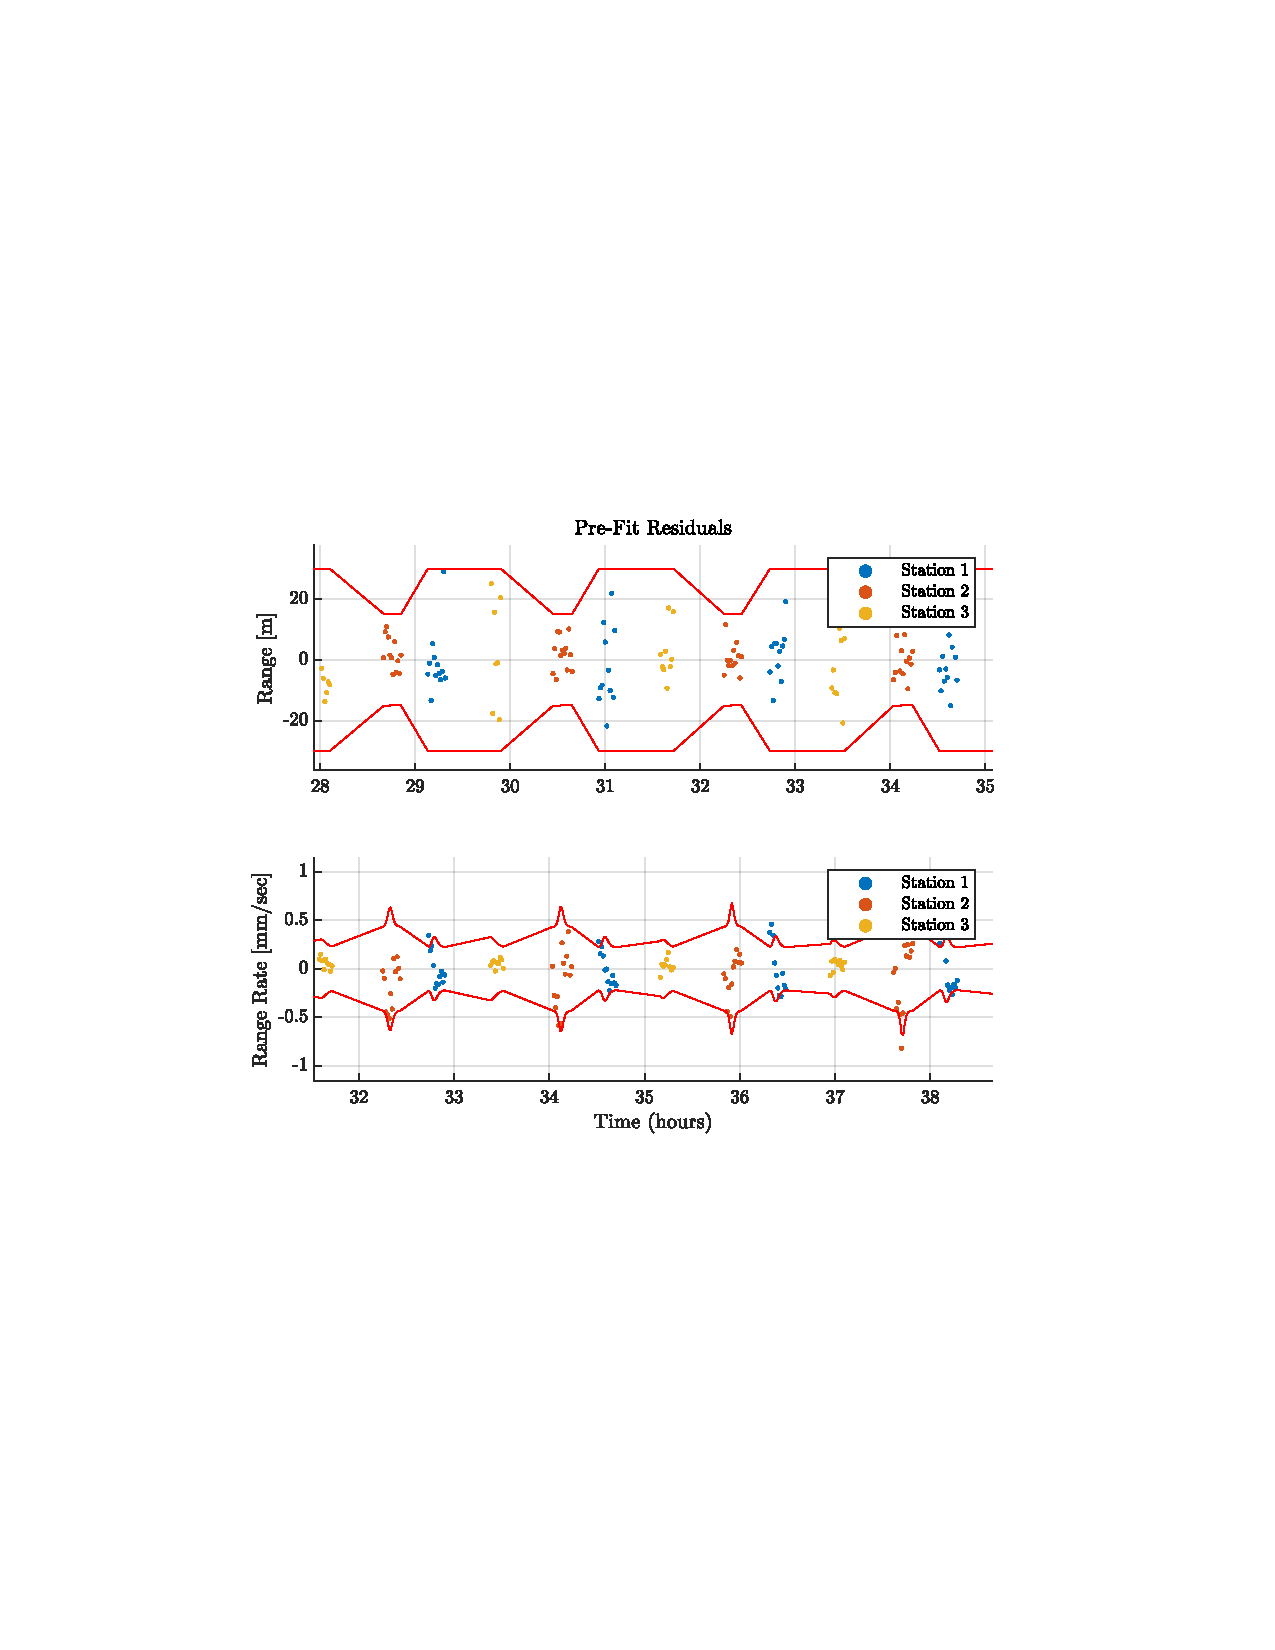
\includegraphics[clip,trim=4cm 8.5cm 4cm 8.5cm, width=.5\textwidth]{figs/prefit_res_zoom1_final.pdf}
	\caption{A zoomed for clarity view of the prefit measurement residuals for range (top) and range-rate (bottom).}
	\label{fig:prefit_zoom1}
\end{figure}

%\begin{figure}[!htb]
%	\centering
%	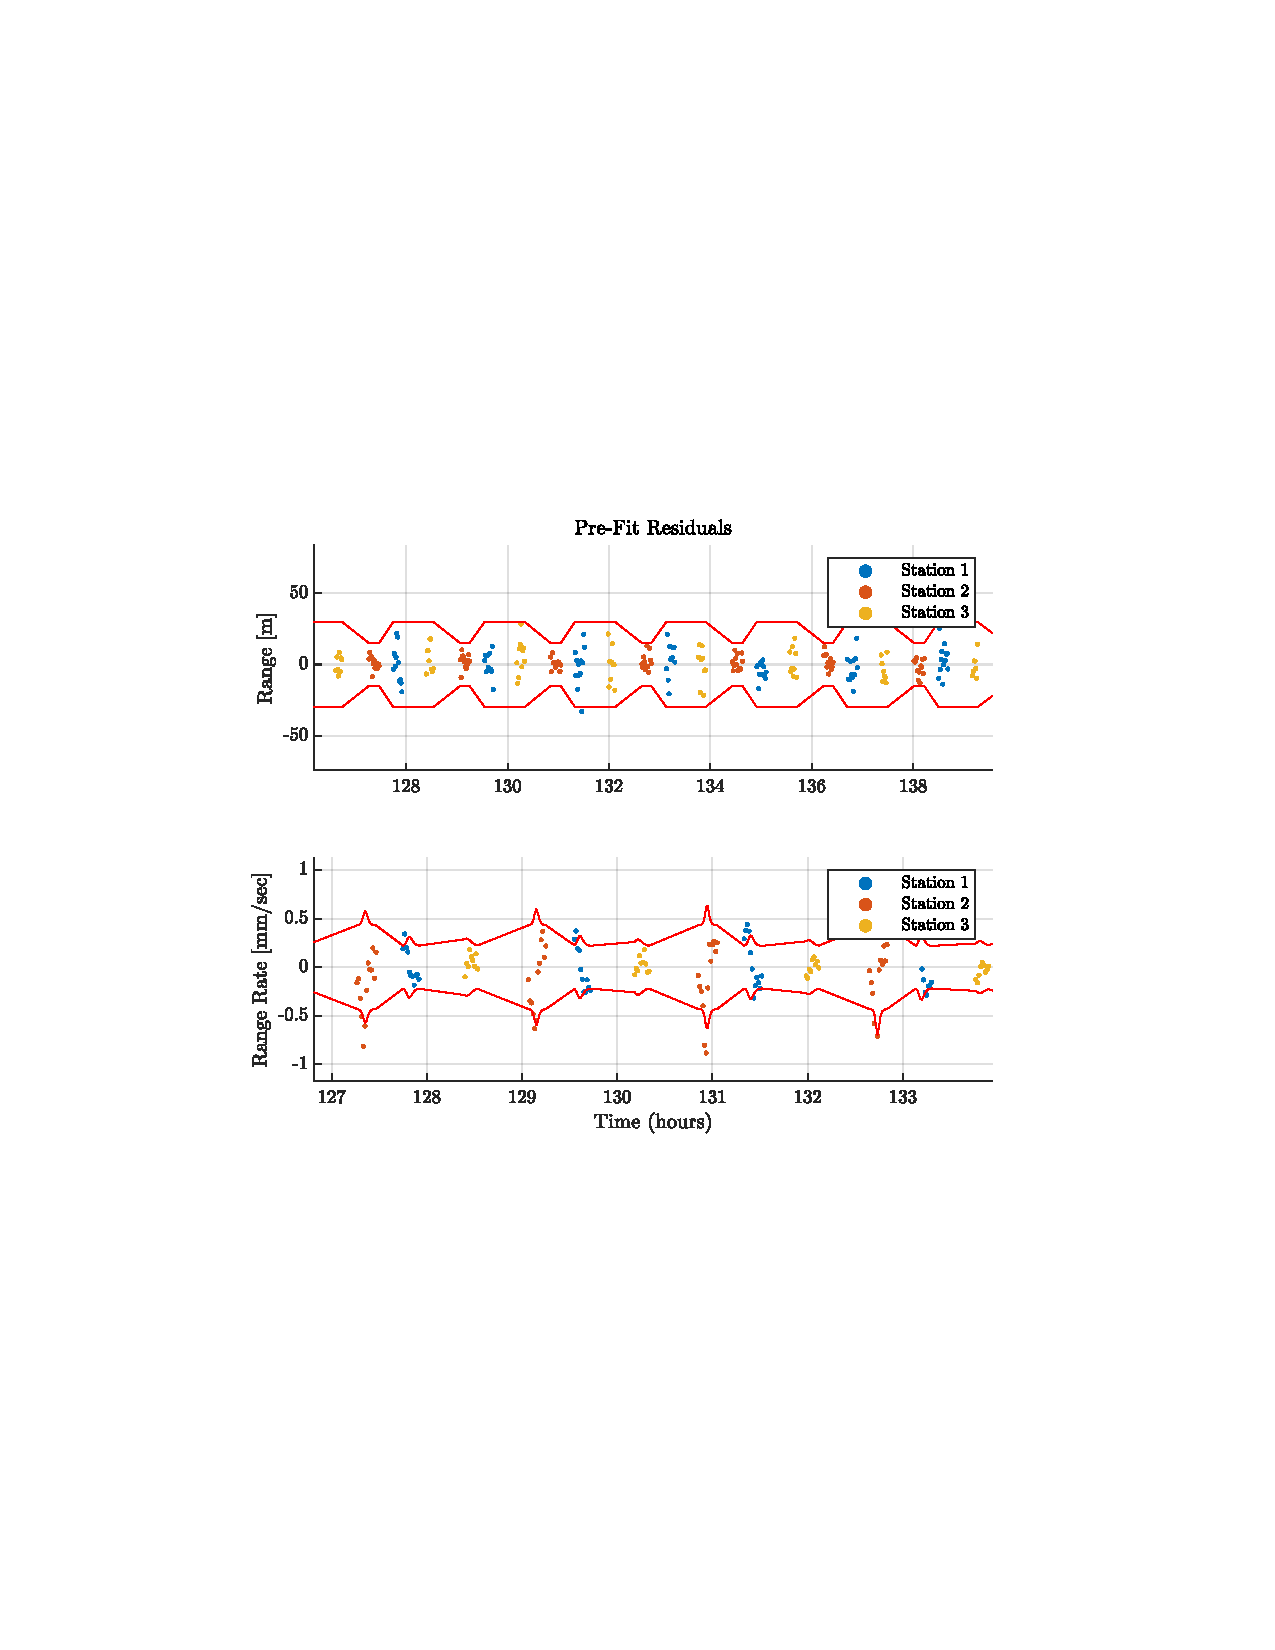
\includegraphics[clip,trim=4cm 8.5cm 4cm 8.5cm, width=.5\textwidth]{figs/prefit_res_zoom2_final.pdf}
%	\caption{A zoomed for clarity view of the prefit measurement residuals for range (top) and range-rate (bottom).}
%	\label{fig:prefit_zoom2}
%\end{figure}

\subsection{Postfit Residuals}

Figure \ref{fig:postfit} shows the postfit measurement residuals when all measurement types and sensors are considered. To better demonstrate detail Figure \ref{fig:postfit_zoom} shows a zoomed-in plot of the measurement residuals.

\begin{figure}[!htb]
	\centering
	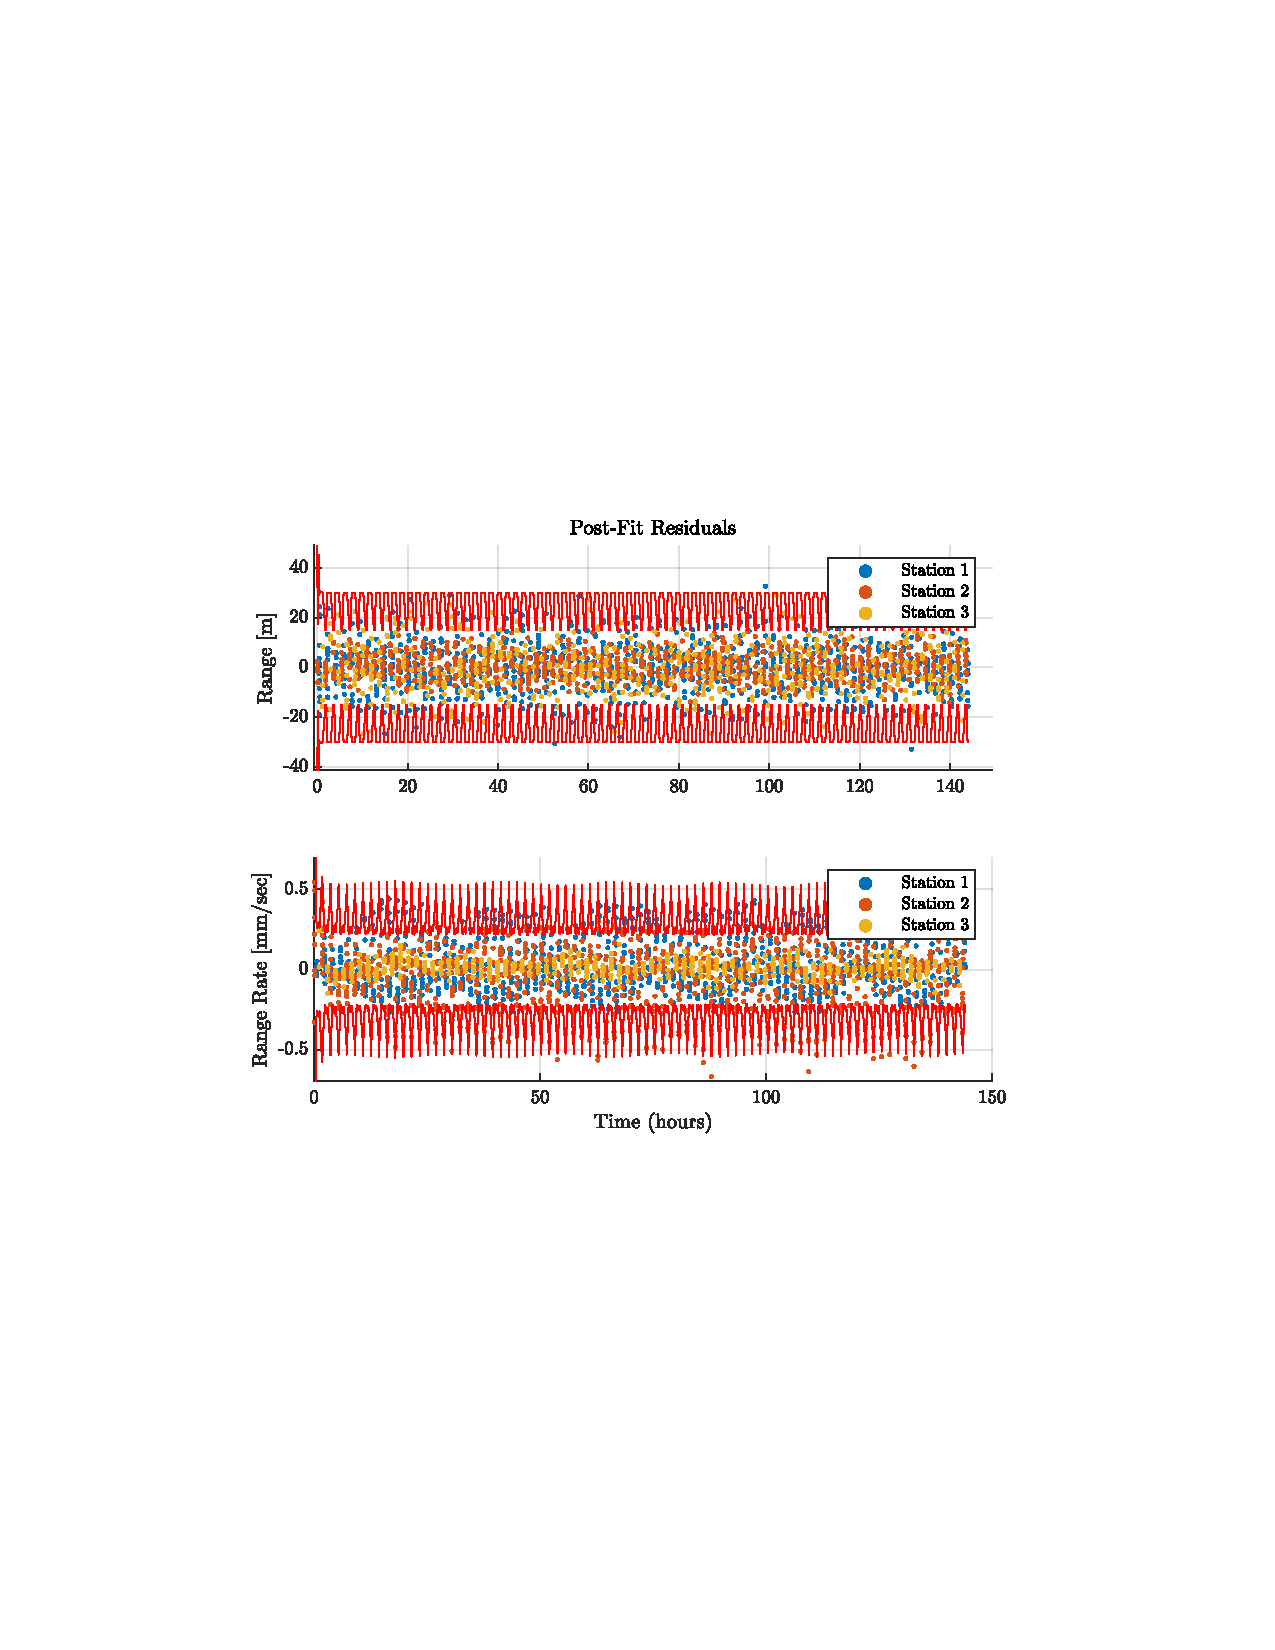
\includegraphics[clip,trim=4cm 8.5cm 4cm 8.5cm, width=.5\textwidth]{figs/postfit_res_final.pdf}
	\caption{The postfit measurement residuals for range (top) and range-rate (bottom).}
	\label{fig:postfit}
\end{figure}

\begin{figure}[!htb]
	\centering
	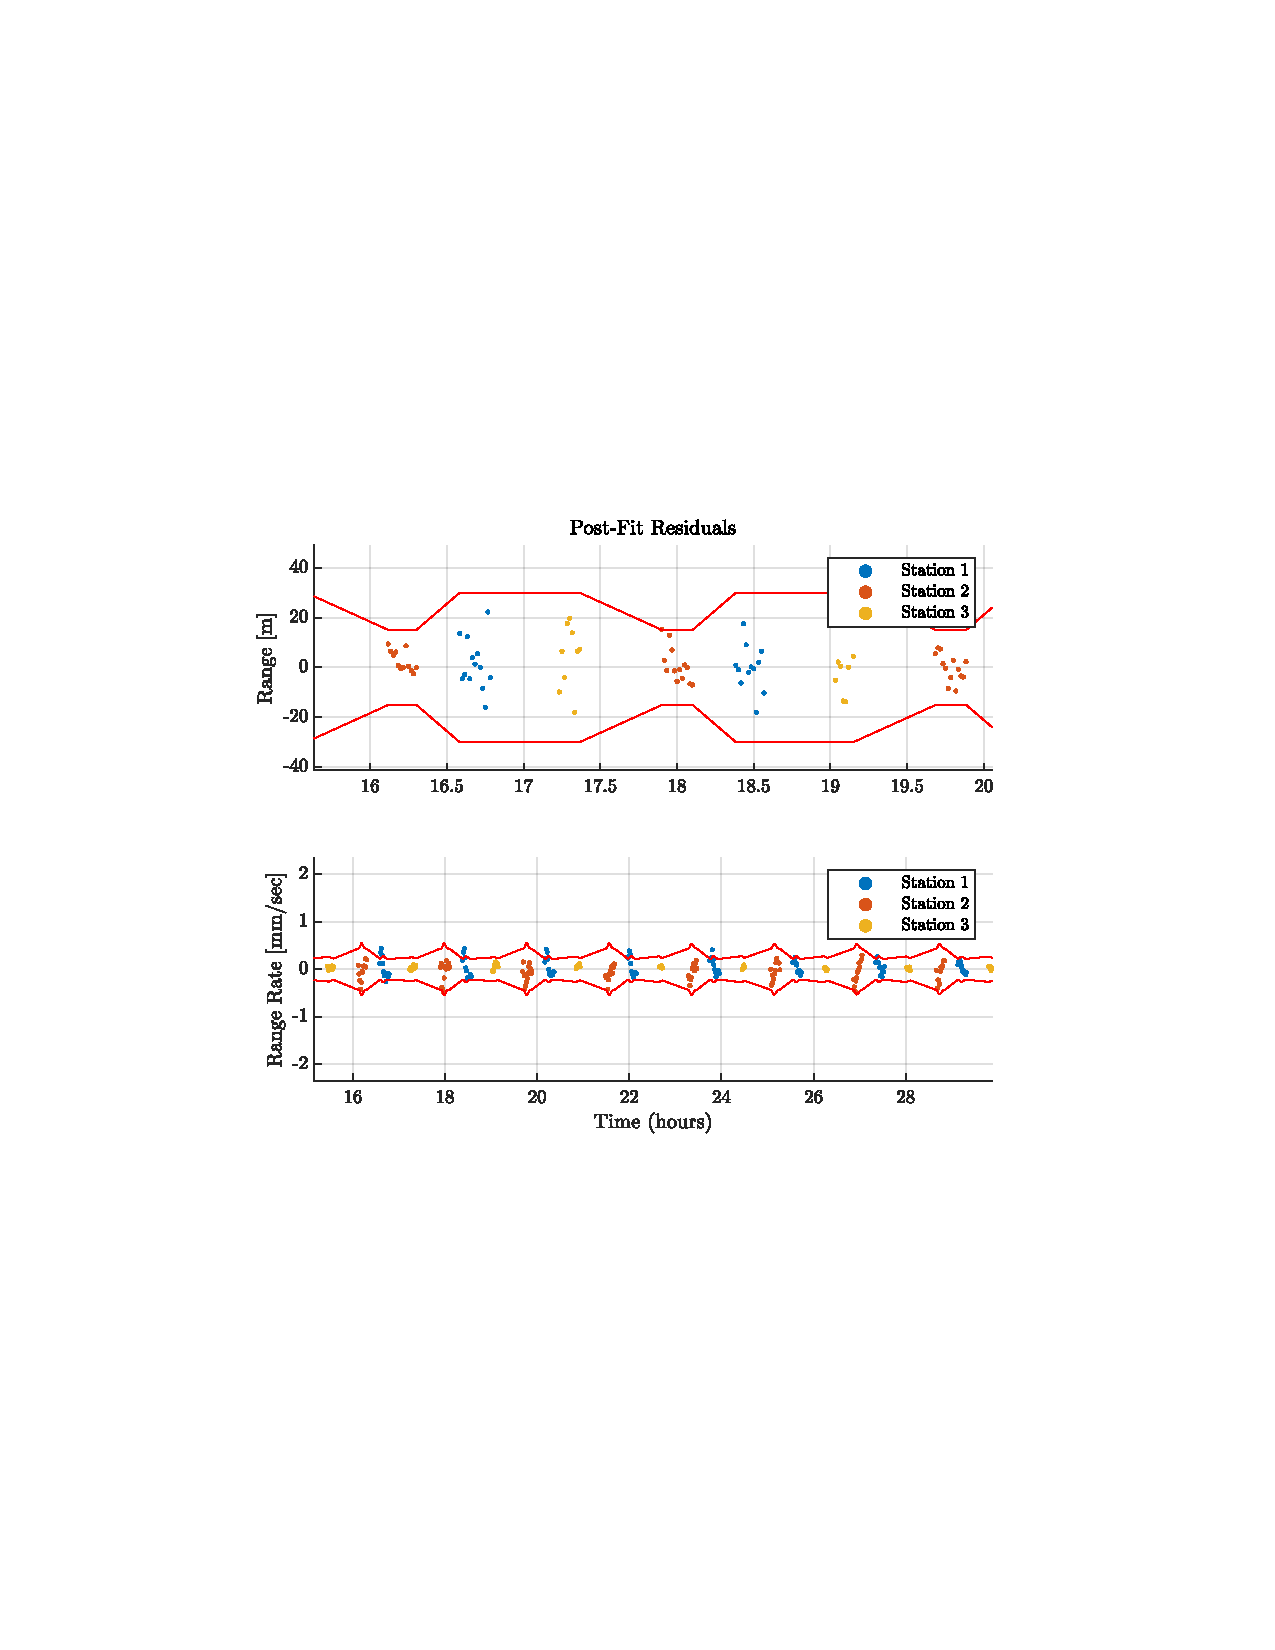
\includegraphics[clip,trim=4cm 8.5cm 4cm 8.5cm, width=.5\textwidth]{figs/postfit_res_zoom1_final.pdf}
	\caption{A zoomed for clarity view of the postfit measurement residuals for range (top) and range-rate (bottom).}
	\label{fig:postfit_zoom}
\end{figure}

\subsection{State Estimates at $\Delta V_1$}

To investigate the consistency of the estimates, case F (all data and all sensors) was designated as the best estimated trajectory. A transformation was found to map vectors into the Radial-Intrack-Crosstrack (RIC) coordinate frame described by the best estimate. For each case, the associated deviation from best-estimate and estimate covariance was transformed into the RIC frame. Figures \ref{fig:rad_cross}, \ref{fig:rad_in}, and \ref{fig:cross_in} showcase these deviations and covariances. \\

Note that the estimates for cases B, F, and G align very well and are difficult to distinguish.

\begin{figure}[!htb]
	\centering
	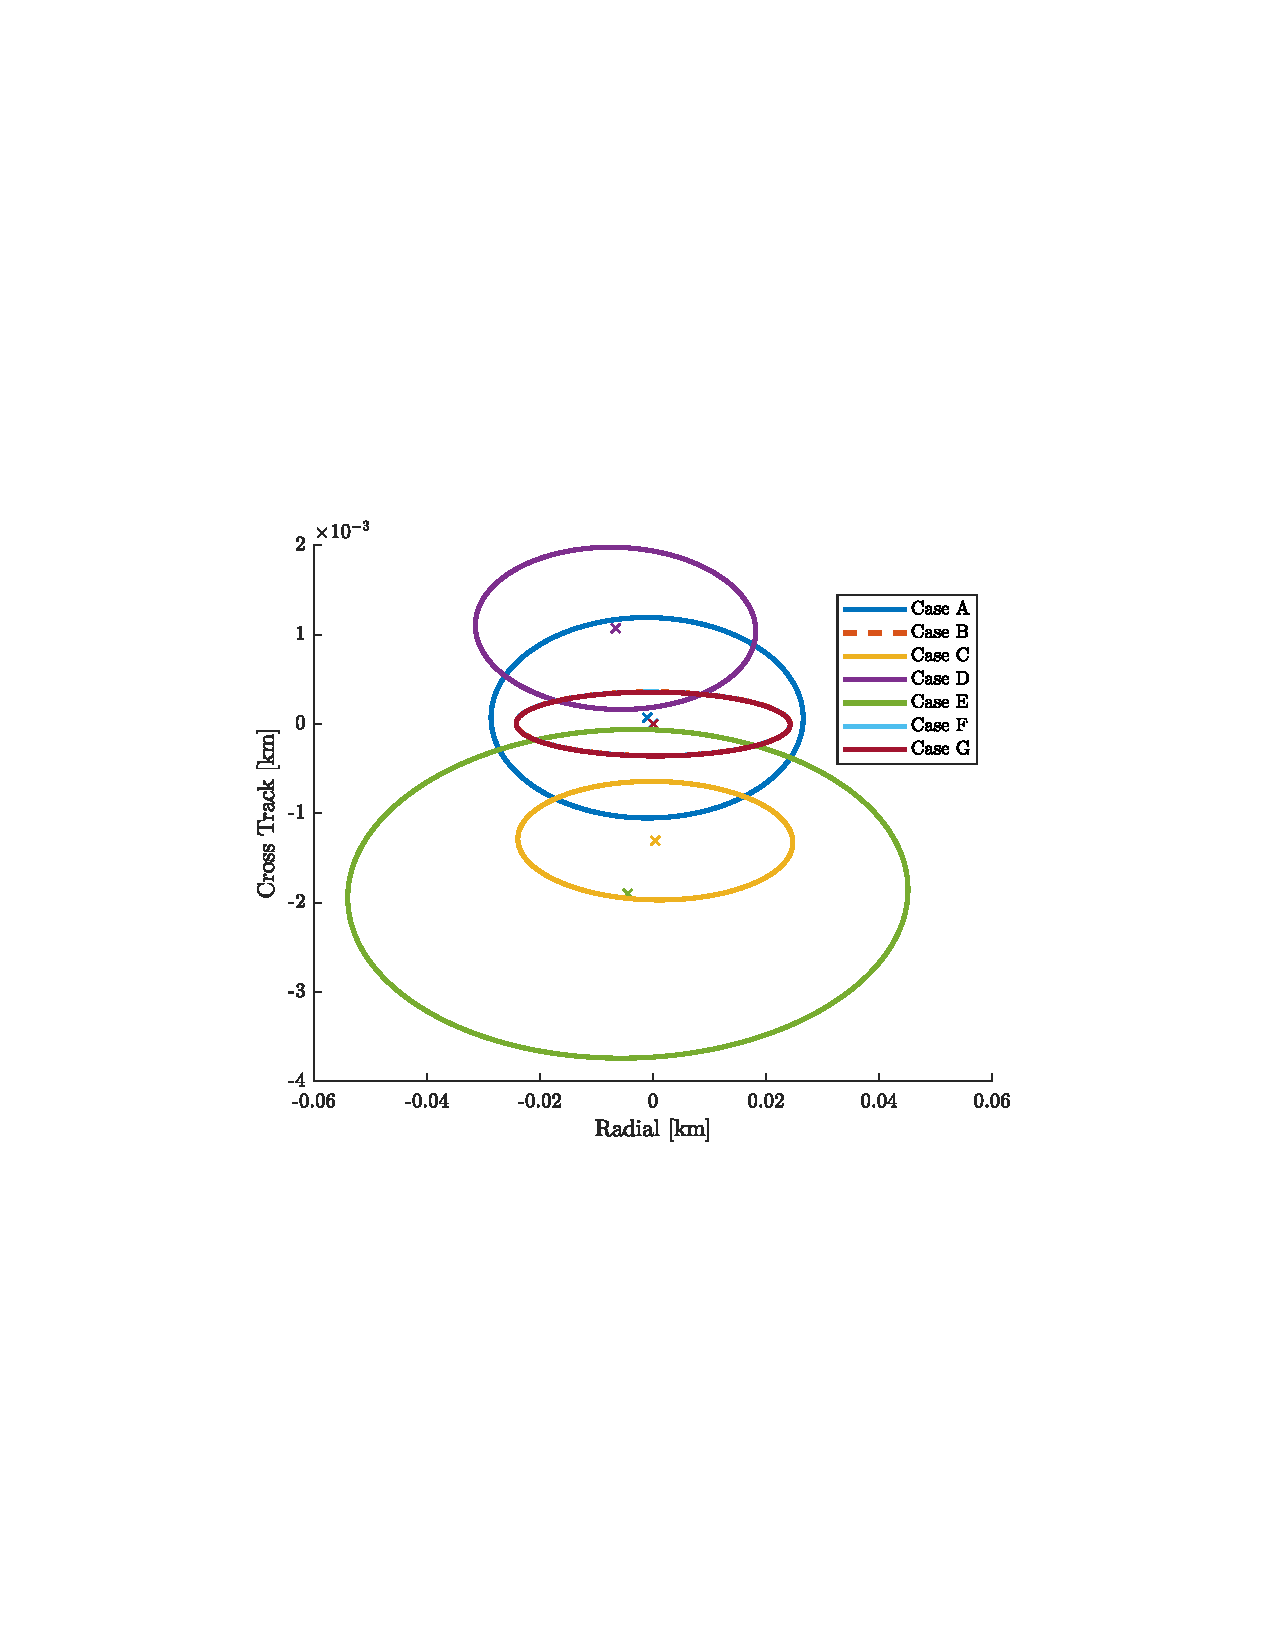
\includegraphics[clip,trim=4cm 8.5cm 4cm 8.5cm, width=.5\textwidth]{figs/RC_final.pdf}
	\caption{The $\Delta V_1$ state estimates for each case expressed in the RIC frame defined by the best estimate. Shown here is a 2D slice of the estimates in the radial and crosstrack directions. The covariance ellipse is $3\sigma$.}
	\label{fig:rad_cross}
\end{figure}

\begin{figure}[!htb]
	\centering
	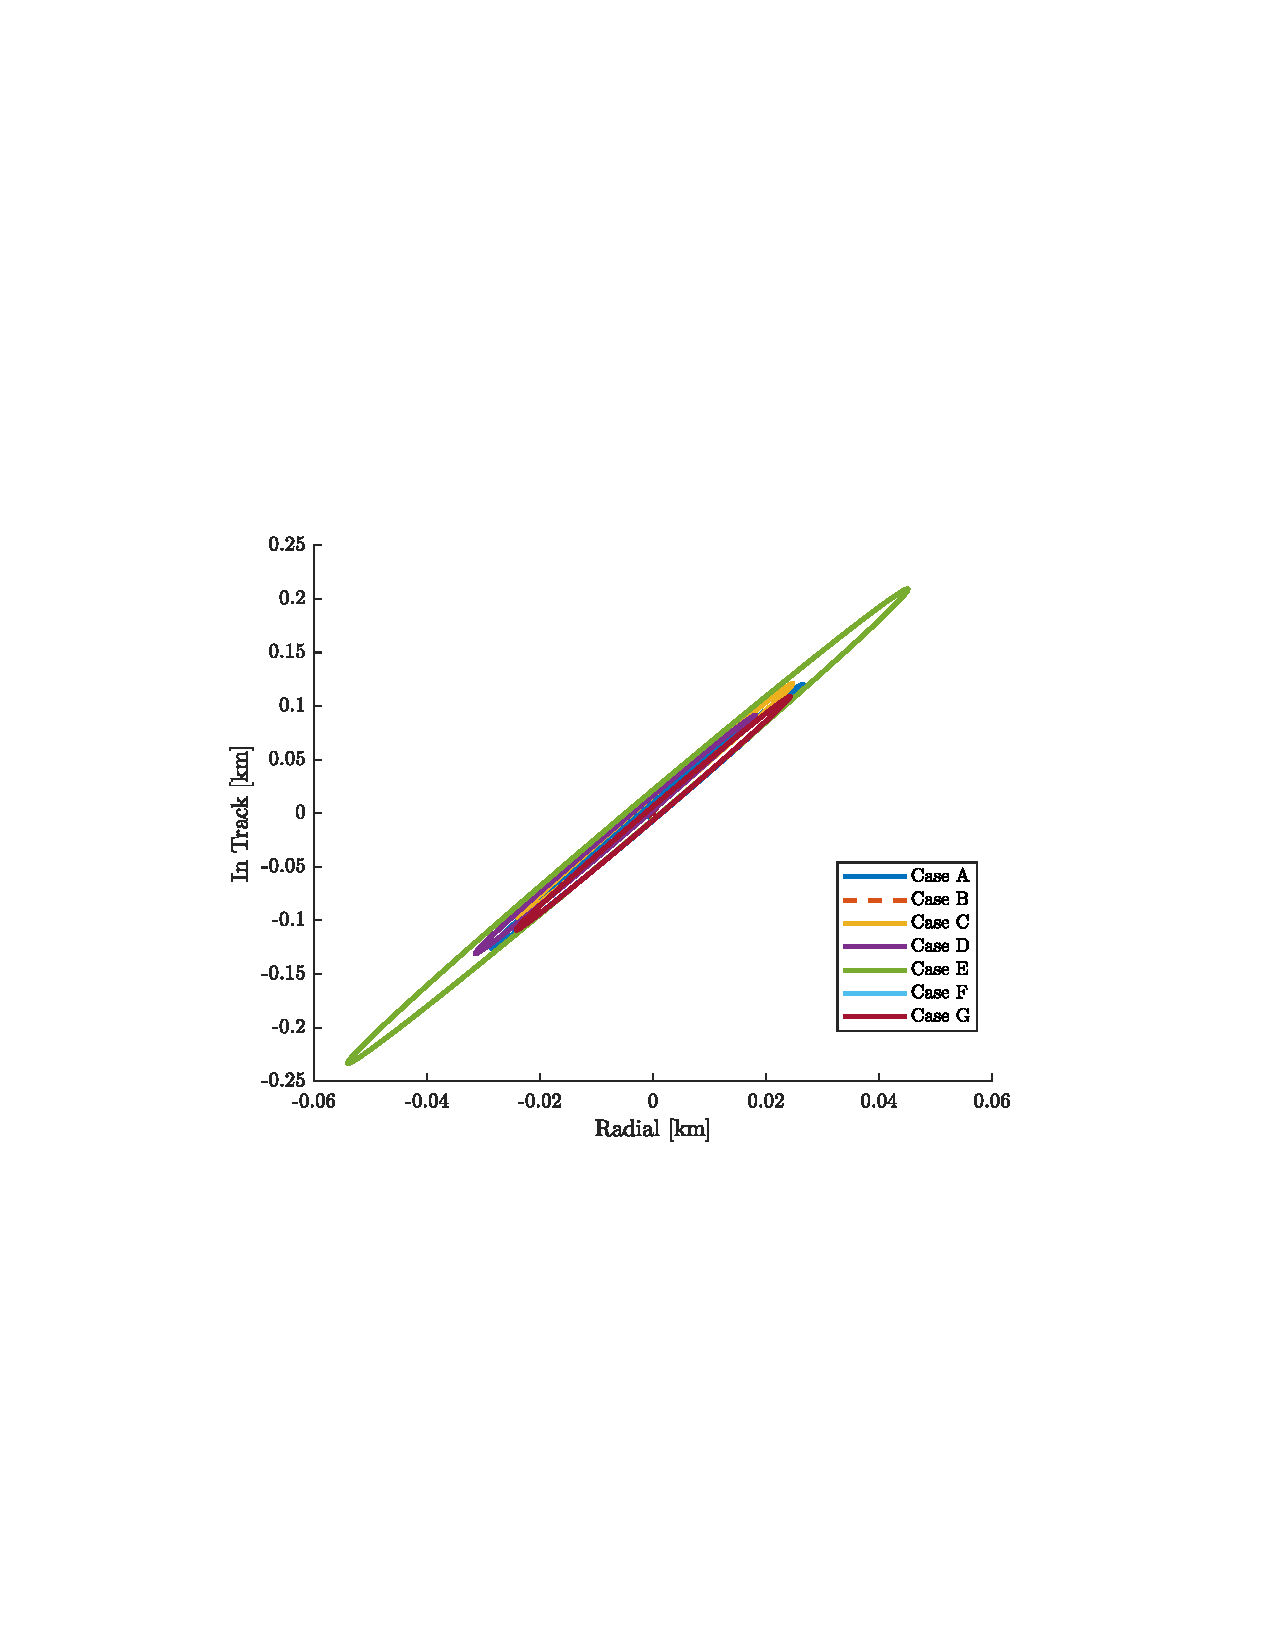
\includegraphics[clip,trim=4cm 8.5cm 4cm 8.5cm, width=.5\textwidth]{figs/RI_final.pdf}
	\caption{The $\Delta V_1$ state estimates for each case expressed in the RIC frame defined by the best estimate. Shown here is a 2D slice of the estimates in the radial and intrack directions. The covariance ellipse is $3\sigma$.}
	\label{fig:rad_in}
\end{figure}

\begin{figure}[!htb]
	\centering
	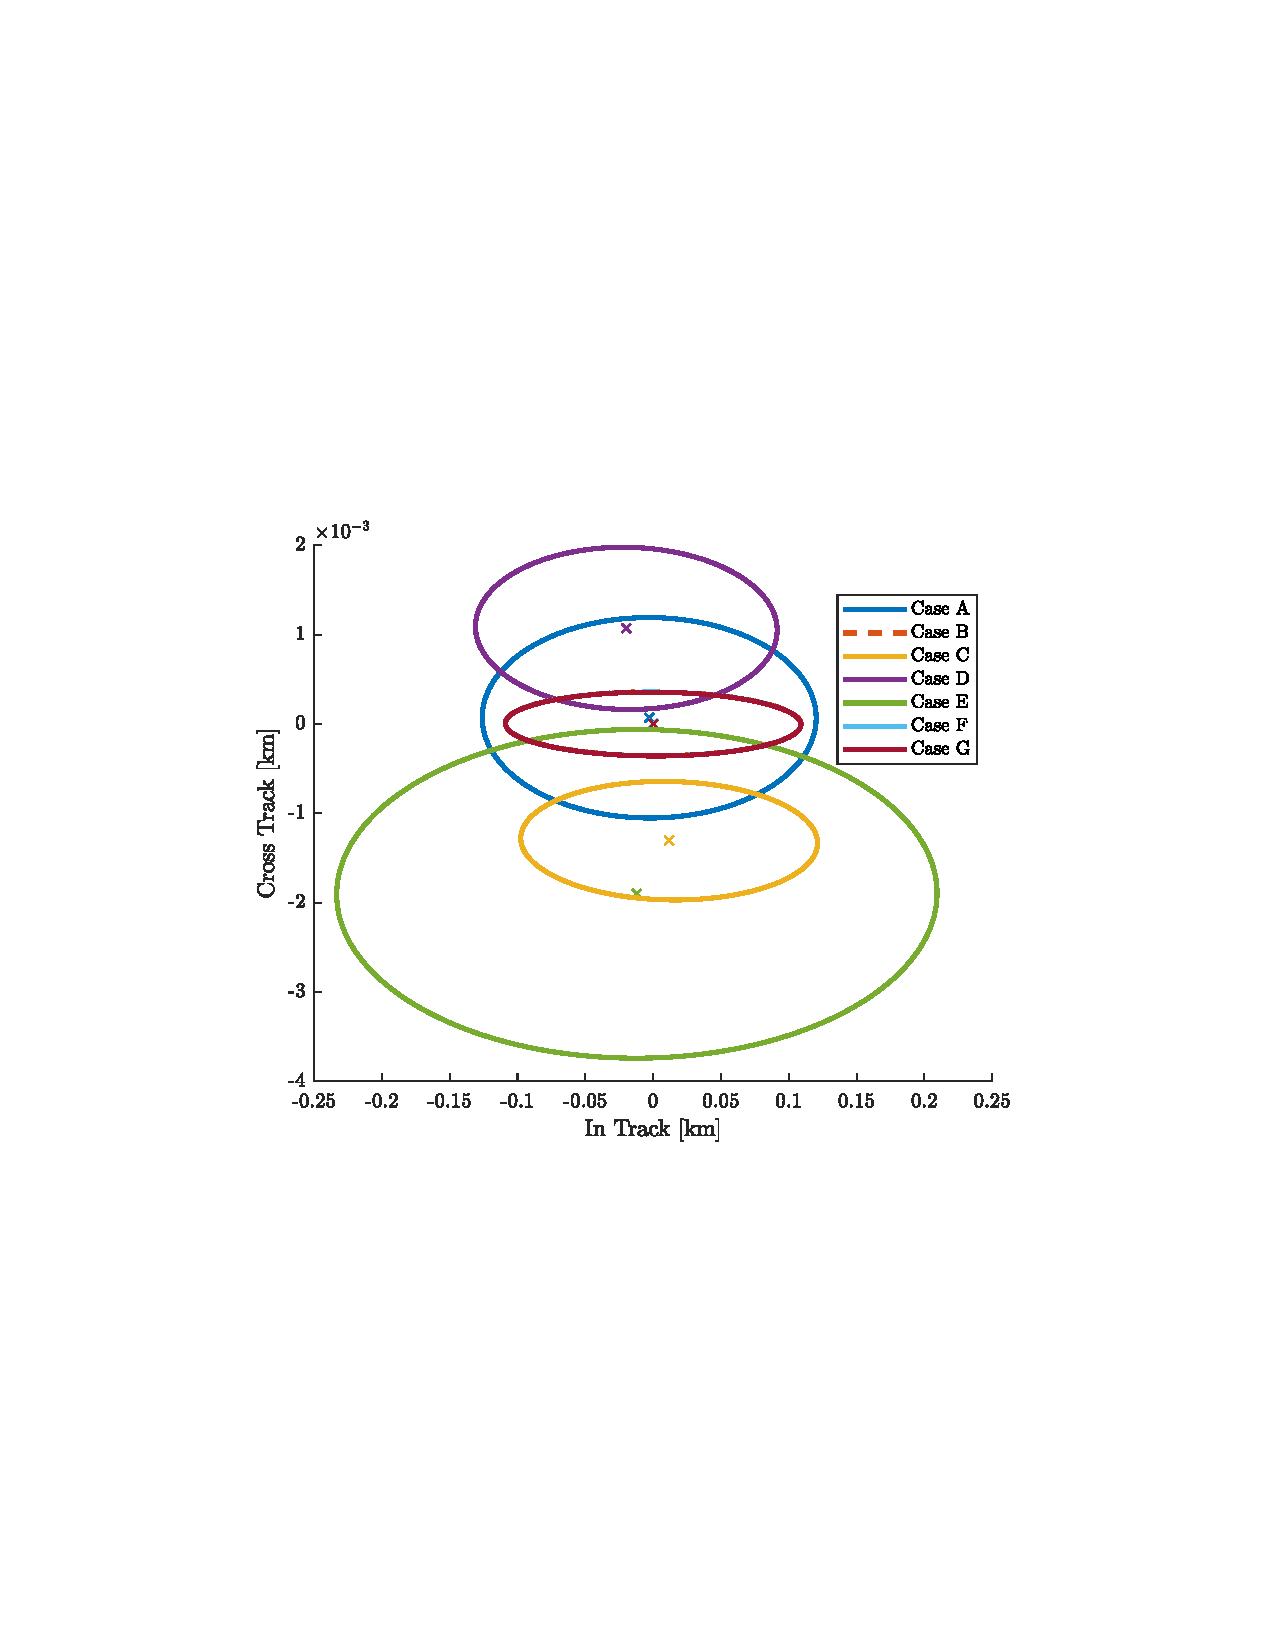
\includegraphics[clip,trim=4cm 8.5cm 4cm 8.5cm, width=.5\textwidth]{figs/CI_final.pdf}
	\caption{The $\Delta V_1$ state estimates for each case expressed in the RIC frame defined by the best estimate. Shown here is a 2D slice of the estimates in the intrack and crosstrack directions. The covariance ellipse is $3\sigma$.}
	\label{fig:cross_in}
\end{figure}

\section{Discussion}

We can form a variety of conclusions from the deliverables. We begin with a discussion of the residuals. First we note that residuals at the beginning of the epoch are high, this indicates that our LM optimization scheme has most likely not provided us an accurate initial state estimate. Despite this, the UKF is able to recover from these initial errors and converge to an estimate. We also note that residuals are high immediately after a measurement gap; this is expected. Any estimation error immediately before a measurement gap is bound to grow during the nonlinear orbital propagation without any updates. Even if we had perfect estimation, error is bound to grow due to the unmodeled dynamics of our system. It is possible that our simplifications in dynamics modeling are contributing significantly to the growth of these residuals. We may be able to increase estimator performance by increasing the fidelity of our drag and SRP models. The frequency with which the range rate residuals exceed their $3\sigma$ bounds is also unexpected. This indicates some inaccuracy in the measurement or dynamics modeling. \\

There is some periodicity in the residuals with a period of approximately 24 hours. I expect that this is due to inaccuracies in the ECI to ECEF transformation. When investigating the zoomed in segments of the residuals we see that the range residuals are approximately white while the range rate ones appear to have some structure. If my modeling and code was perfect, both would appear white. This indicates there is some error in the way range-rate measurements are predicted. The range rate measurement is very sensitive, so it is likely that the same ECI to ECEF transformation errors identified previously are also contributing to this structure. \\

Figure \ref{fig:res_change} shows the difference between prefit and postfit residuals. These changes do not go to zero, which is considered a good thing as it implies the filter is not becoming smug. However, there is more clear 24 hour periodicity evident in this plot. This indicates a flawed ECI to ECEF transformation. Notably, this periodicity is highest for stations 1 and 2. Station 3 is farthest from the equator so it may somehow be least effected by the transformation errors. \\ 

\begin{figure}[!htb]
	\centering
	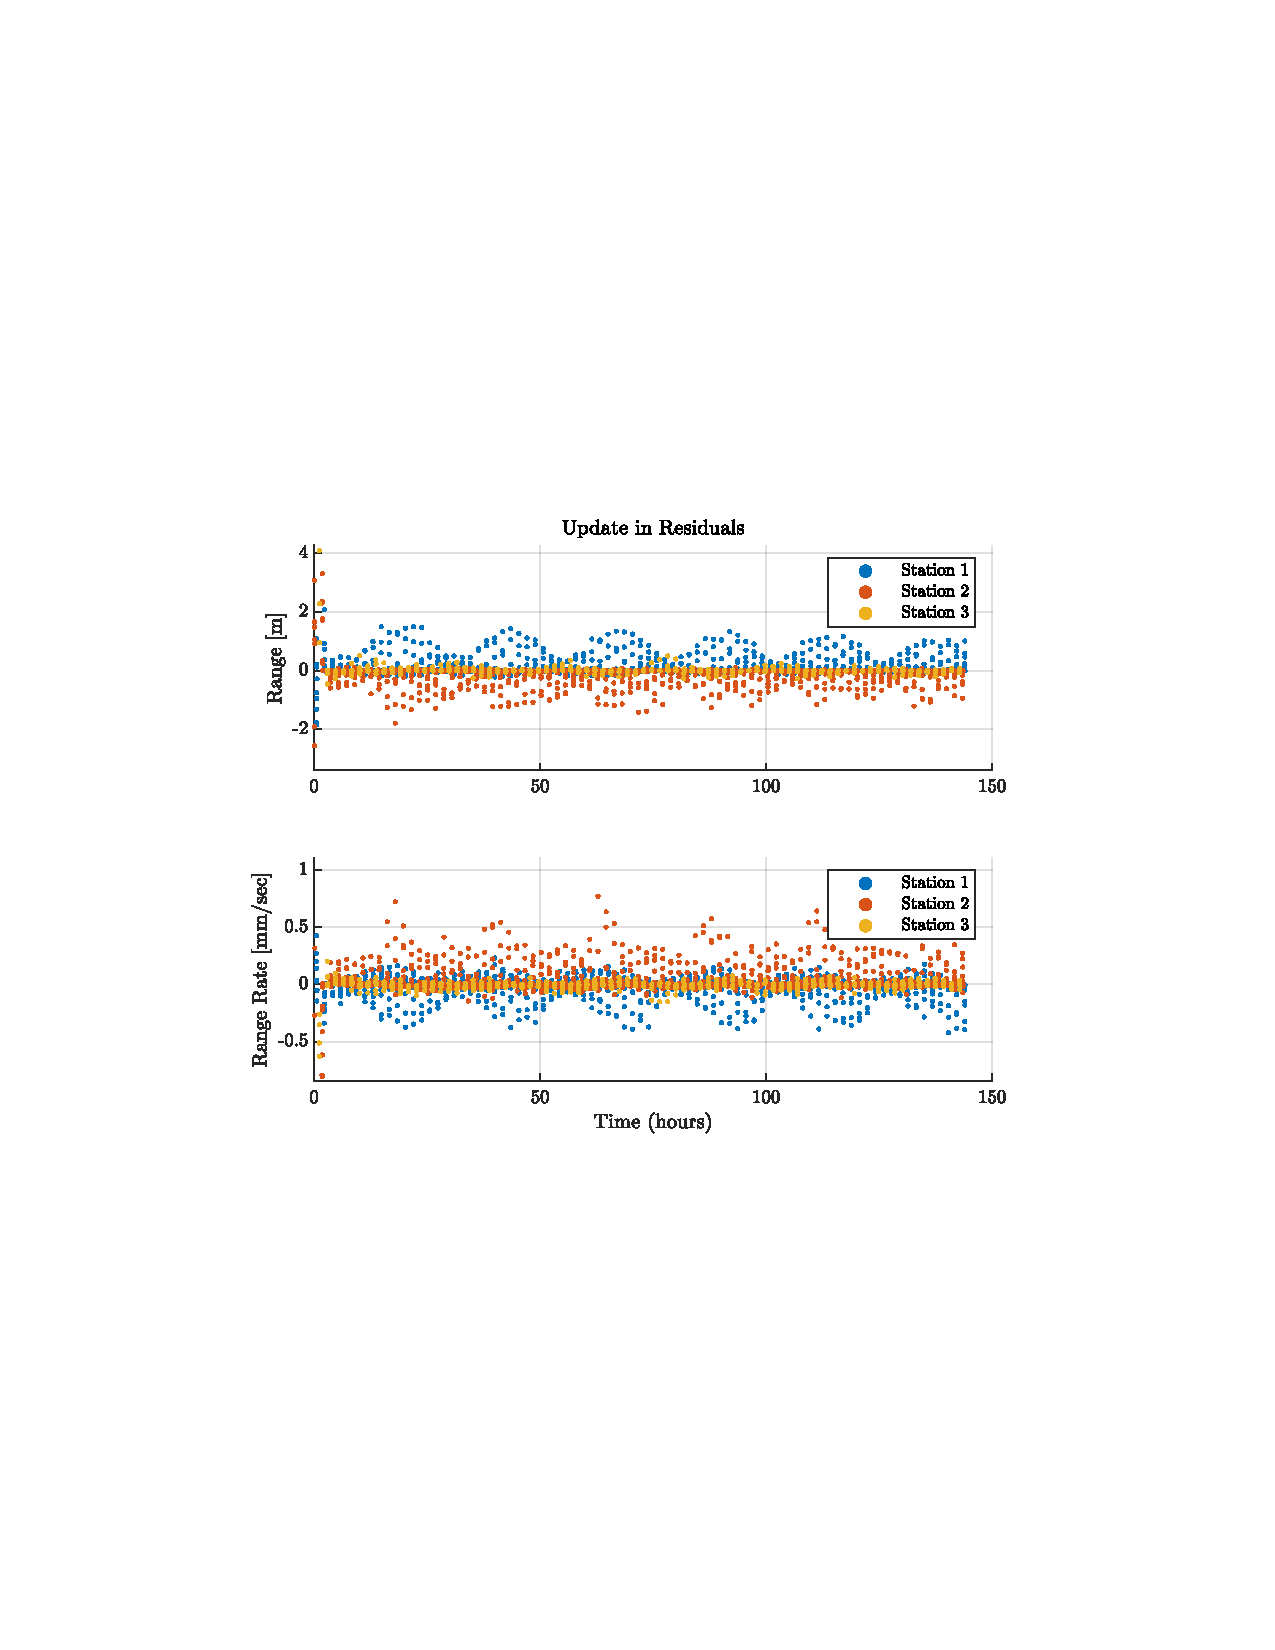
\includegraphics[clip,trim=4cm 8.5cm 4cm 8.5cm, width=.5\textwidth]{figs/update_res.pdf}
	\caption{The difference between prefit and postfit residuals.}
	\label{fig:res_change}
\end{figure}

Dr. Jah has informed us that there is a change in attitude after three days of propagation. A very high fidelity estimator and model would show this change in attitude in changing residuals after three days. I am not able to detect any change in residuals, demonstrating another limitation of my low fidelity modeling. \\

In order to find measurement biases, the system was run while considering measurements from only two of the stations. With this method I was able to detect a range measurement bias of 19.8 meters in station 3. Figure \ref{fig:bias} shows the residuals with a clear bias in station 3. \\

\begin{figure}[!htb]
	\centering
	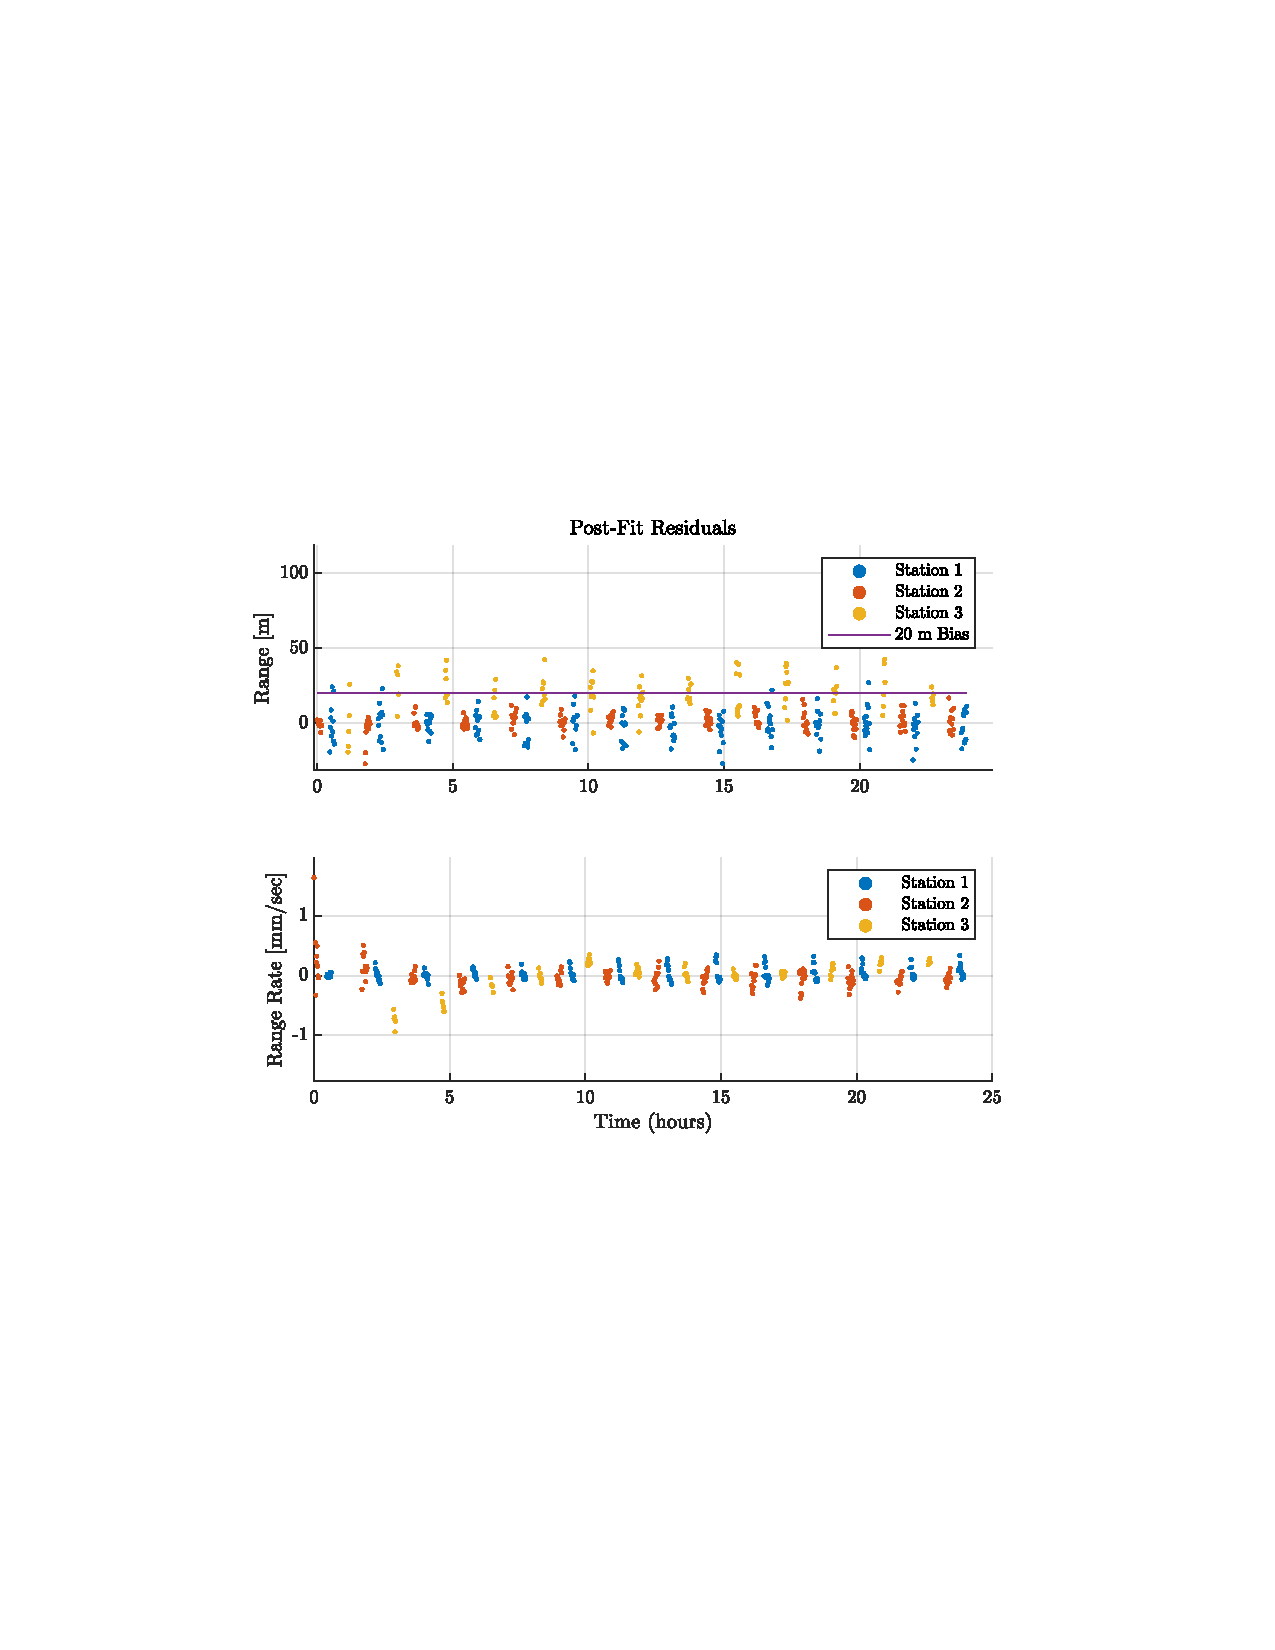
\includegraphics[clip,trim=4cm 8.5cm 4cm 8.5cm, width=.5\textwidth]{figs/bias.pdf}
	\caption{Investigation into the measurement bias. Displayed is a 20 m bias in range which was revealed as the true bias by Dr. Jah.}
	\label{fig:bias}
\end{figure}

Finally, we discuss the plots of our estimates in the RQW coordinate system. This segment of the project involves six day's worth of measurements followed by one days of propagation. We note that the covariance ellipses of all estimates are relatively similar. This is because the process noise injected during a day of propagation is a much larger component of the final uncertainty than the estimate uncertainty after the final measurement is incorporated. \\

Next we note that the estimates and covariances of cases B, F, and G are almost indistinguishable. From this, we can draw two conclusions. First, most of the information content in the estimate comes from range-rate measurements. This is supported by the fact that case A has a similar estimate to these three but a larger covariance. Second, we conclude that information from the first three days of data (before the attitude change), does not contribute significantly to the final estimate (after the attitude change). This provides additional evidence that my estimator is not sensitive enough to detect the attitude change Dr. Jah mentioned. \\

We note that the covariance in Case E is highest. Out of the one station estimates it is followed by cases D and C. This order mirrors the order in which the stations are utilized at the end of measurement. Station 1 is last, Station 2 is second to last, and Station 3 is third to last. Therefore it makes sense that the covariance of these estimates would be ordered in the way they are because estimates with a longer time since measurement have a larger covariance. 

\section{Conclusion}

In conclusion, we have demonstrated a modest estimation scheme with plenty of room for improvement. While estimates of satellite state at the delivery time are provided, analysis of measurement residuals and the consistency of these estimates suggests there is room for improvement in measurement and dynamics modeling. \\

\newpage
\appendix
\section{Code}

\subsection{\texttt{main.cc}}
\lstinputlisting{../../src/project/main.cc}

%%plot matlab files now
%\lstset { %
%	language=matlab,
%	backgroundcolor=\color{black!5}, % set backgroundcolor
%	basicstyle=\tiny,% basic font setting
%}

\subsection{\texttt{VehicleState.h}}
\lstinputlisting{../../src/project/VehicleState.h}

\subsection{\texttt{Estimators.h}}
\lstinputlisting{../../src/project/Estimators.h}

\subsection{\texttt{Util.h}}
\lstinputlisting{../../src/project/Util.h}

\subsection{\texttt{VehicleState.cc}}
\lstinputlisting{../../src/project/VehicleState.cc}

\subsection{\texttt{Estimators.cc}}
\lstinputlisting{../../src/project/Estimators.cc}

\subsection{\texttt{Util.cc}}
\lstinputlisting{../../src/project/Util.cc}

\end{document}
